\documentclass{neu_handout}
\usepackage{url}
\usepackage{amssymb}
\usepackage{amsmath}
\usepackage{marvosym}
\usepackage{graphicx}
\usepackage[pdftex]{graphicx}
\usepackage{subfigure}
\graphicspath{ {images/} }
\everymath{\displaystyle}

% Professor/Course information
\title{Homework 5}
\author{Emily Dutile}
\date{April 2018}
\course{CS7295}{Info Viz}

\begin{document}

The dataset used for this assignment can be found here \footnote{\url{https://catalog.data.gov/dataset/energy-generation-by-state-and-technology-2009}}.

\section*{1 Dear Data}

\subsection*{1.1 My Visualization}


\begin{figure}[h]
\centering
{
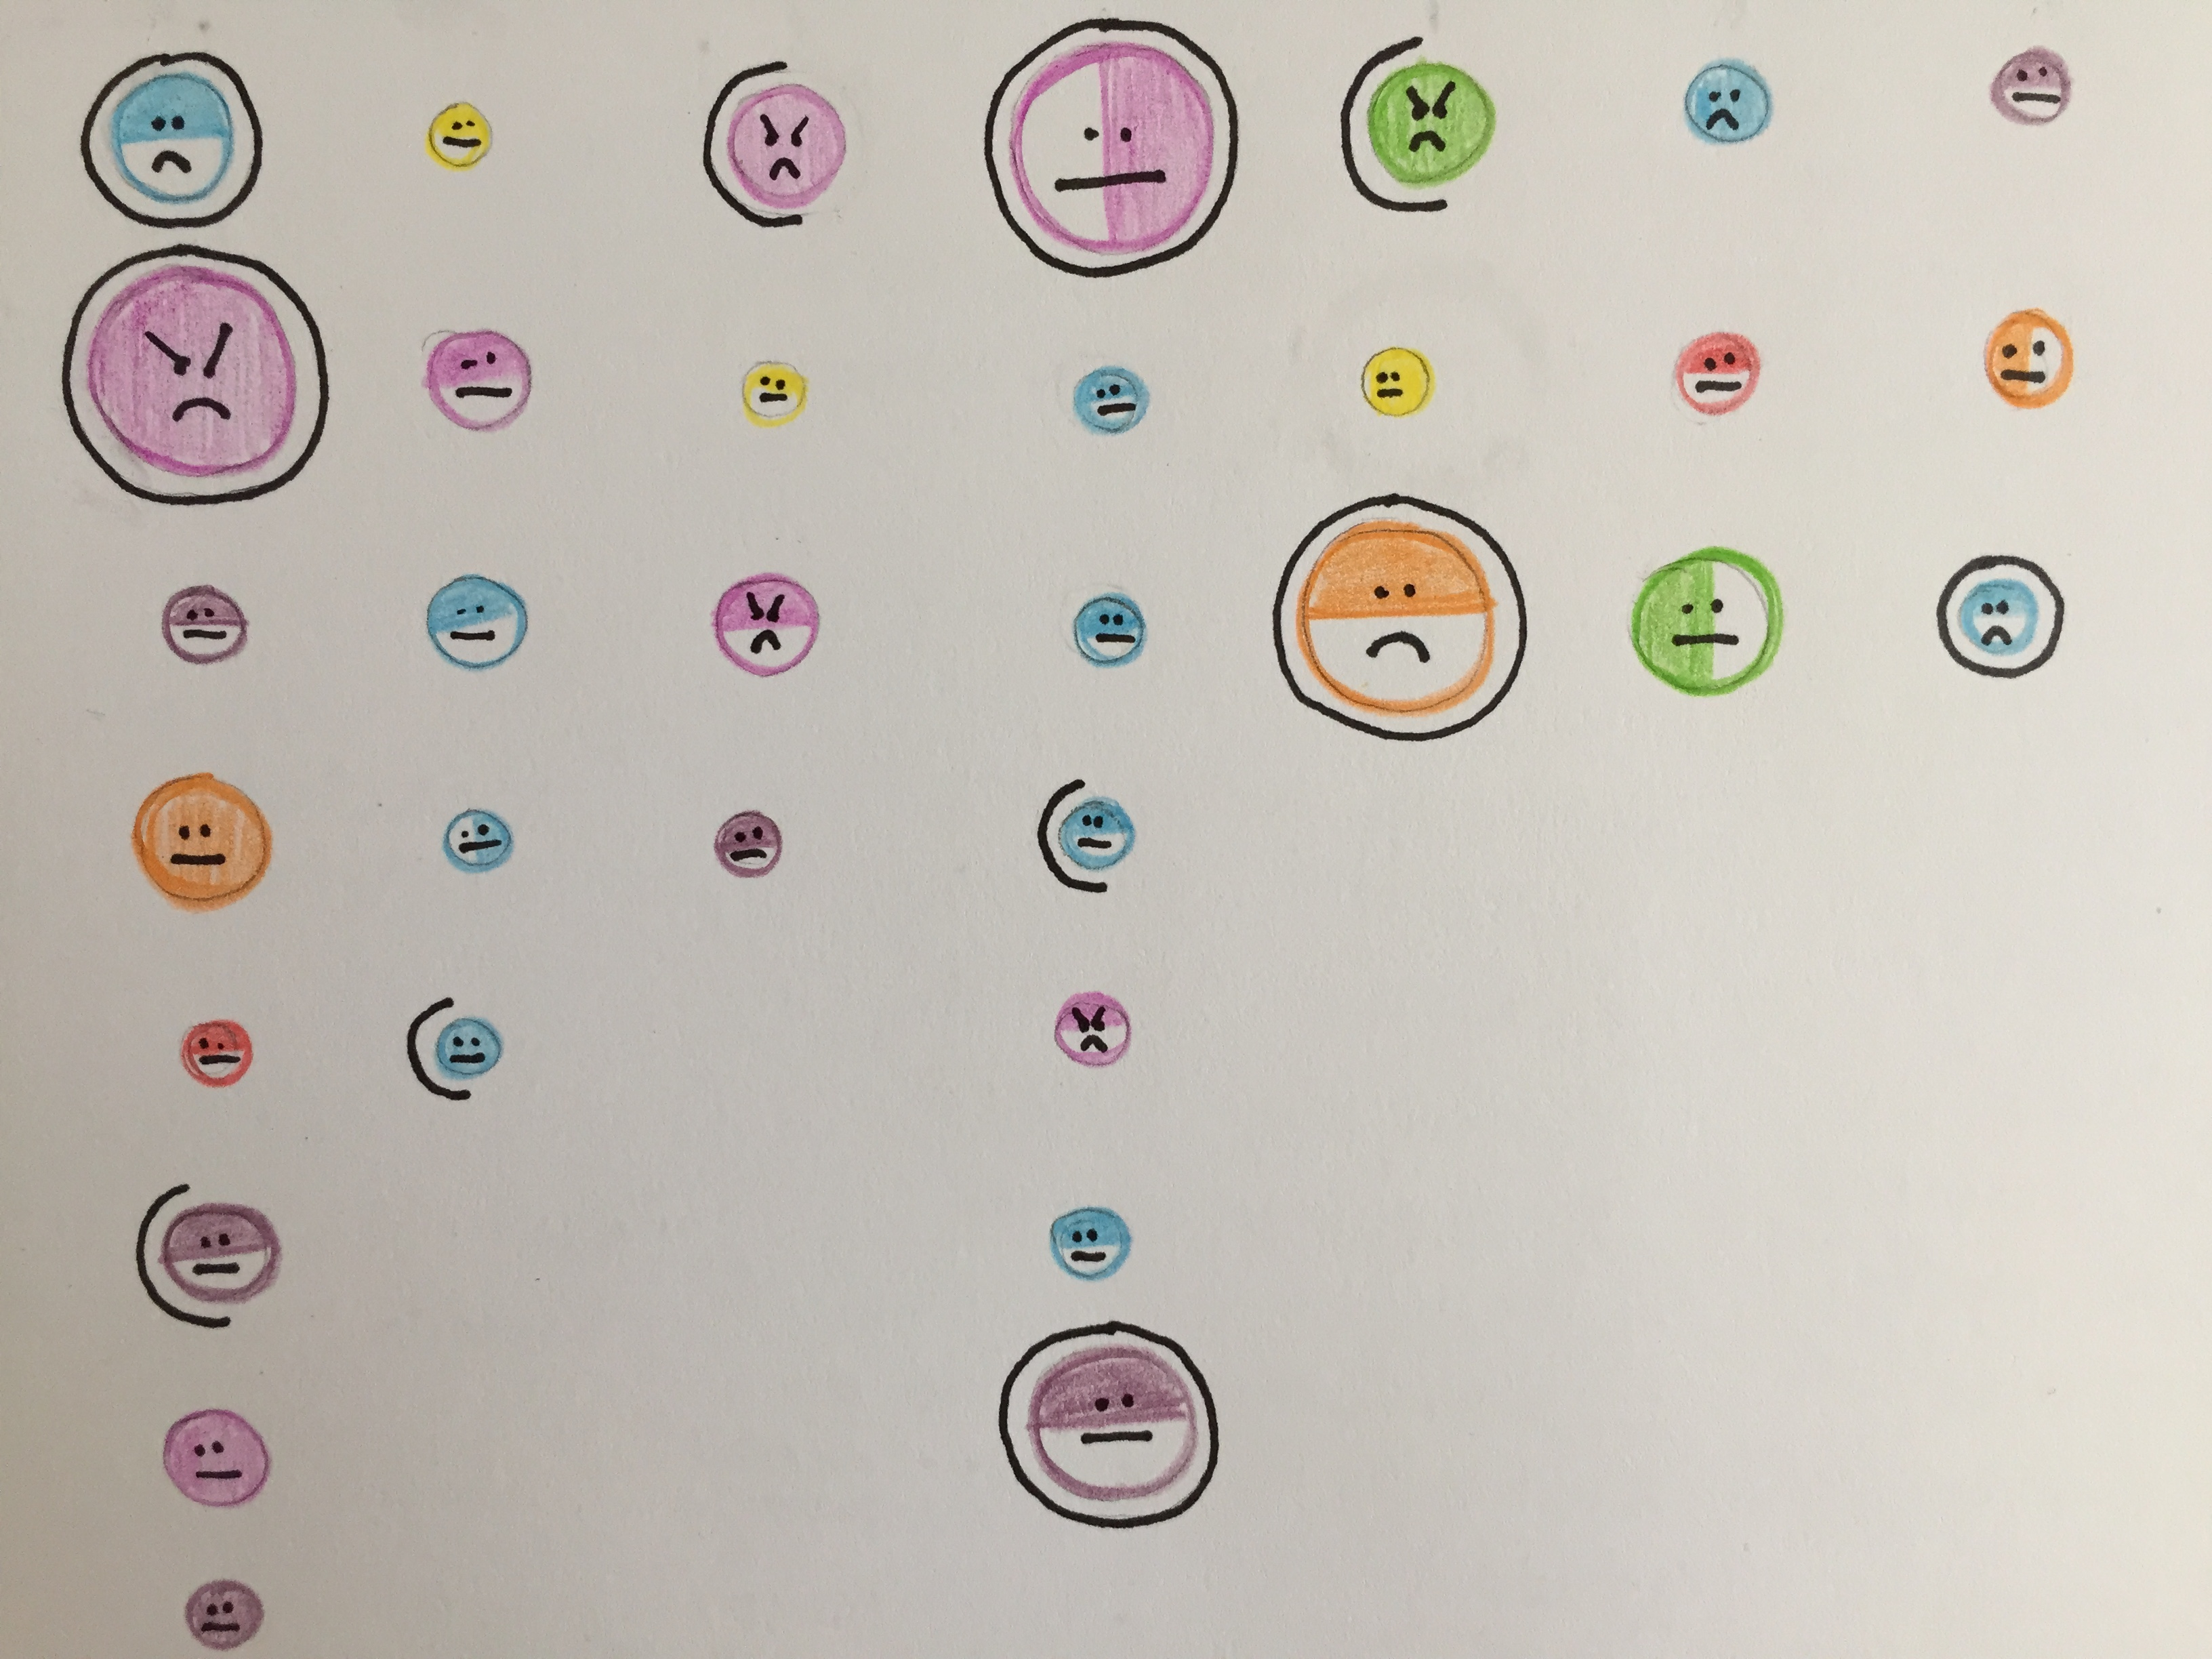
\includegraphics[width=0.4\linewidth]{myviz1}
}
{
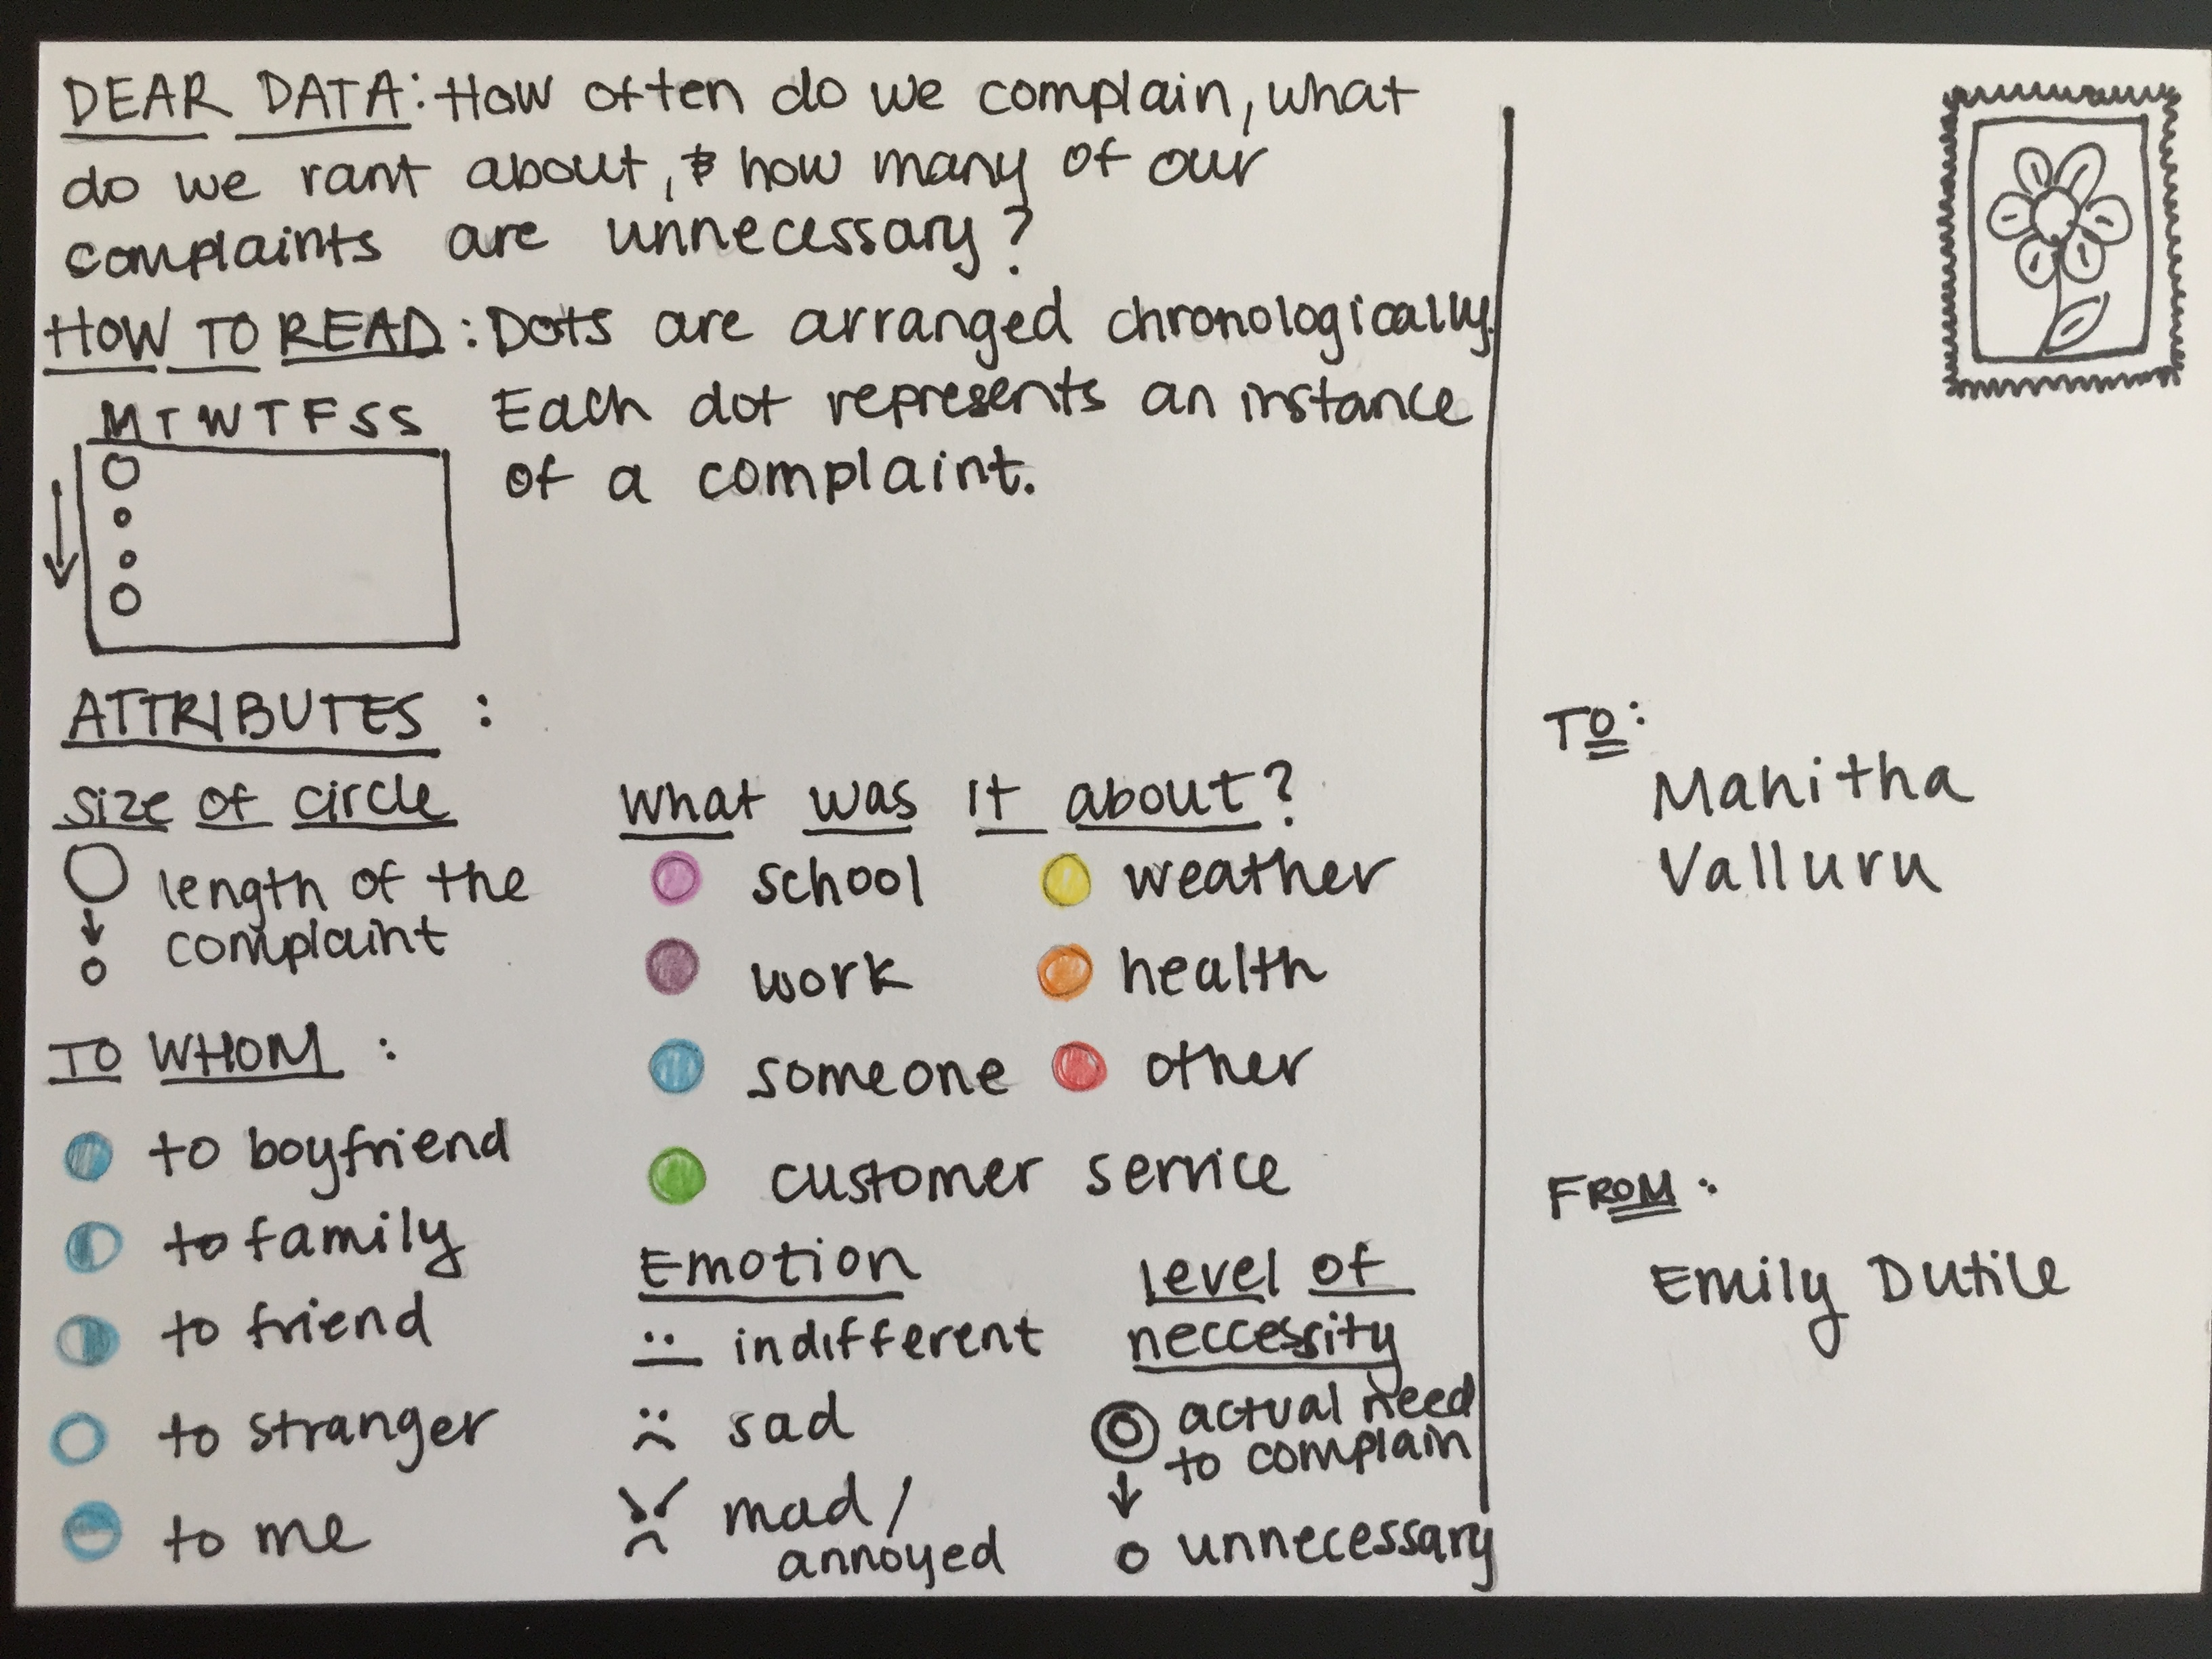
\includegraphics[width=0.4\linewidth]{myviz2}
}
\end{figure}

My dear data assignment was to analyze how often I/we complain, what do I/we rant about, and how many of my/our complaints are unnecessary. I decided to keep track of each instance that I caught myself or someone else complaining. I wanted to see whether it was me who complains a lot to others, or do I allow others to complain a lot to me. Any time I/someone else expressed annoyance, distastefulness of a situation (unnecessarily), or anything else that resembled a complaint, I kept track of who was doing the complaining, what was the subject, what was the persons emotion, the length of the complaint, and the necessity of the complaint. I was curious to discover if we complain more in certain environments or when we are around certain individuals. I subjectively decided if I thought the complaint was legitimate or if I found it unnecessary (i.e. calling Comcast and asking why they randomly increased fees when you're in a contract is an actual complaint, where as complaining to have 'nothing to wear' to some event is unnecessary and dramatic). I wanted to design a visual model that could easily show the amount of complains with respect to their topics and how necessary they were. I felt that using instances of circles would easily represent each point and giving them different sizes would appropriately show the length and the level of the complaint. Using color, it made it easy to show who's doing the complaining, and the fill represents the listener.\\

In comparison to my HW4 card, I really thought about what I may complain about in a given day which helped me better understand what I thought would be more important data attributes to emphasize. In my first assignment, I had a topic that I didn't necessarily think about all the time. In some ways I felt like I collected too much data, and the visualization became noisy and more difficult to consume with so many colors and points without overly clear cut lines.


\subsection*{1.2 Pen Pal Visualization}

Mahitha Valluru


\section*{2 Brushing and Linking}

URL: https://jsfiddle.net/dutile/vnv7op6s/19/ \\

Focusing on the EIA Generation and Fuel Data, I wanted to look at the net generation (megawatthours) and the total fuel consumption quantity with respect to the number of plants in the state(s). I didn't find it necessary to add any color, besides to the points that the user was brushing over in order to make them stand out. I think a simplistic approach makes the visuals clean and doesn't add noise to the visuals by adding dimensions or colors. Depending on how many data points the user selects, the JS Fiddler viewer is not ideal to view all of the states since they get scrunched together.


\end{document}
